% =========================================================
% TikZ diagram: Interior / Boundary / Exterior Decomposition
% Place: after Theorem (Interior-Boundary-Exterior Decomposition)
% Requires: \usetikzlibrary{calc,arrows.meta,patterns}
% =========================================================

\begin{figure}[h]
\centering
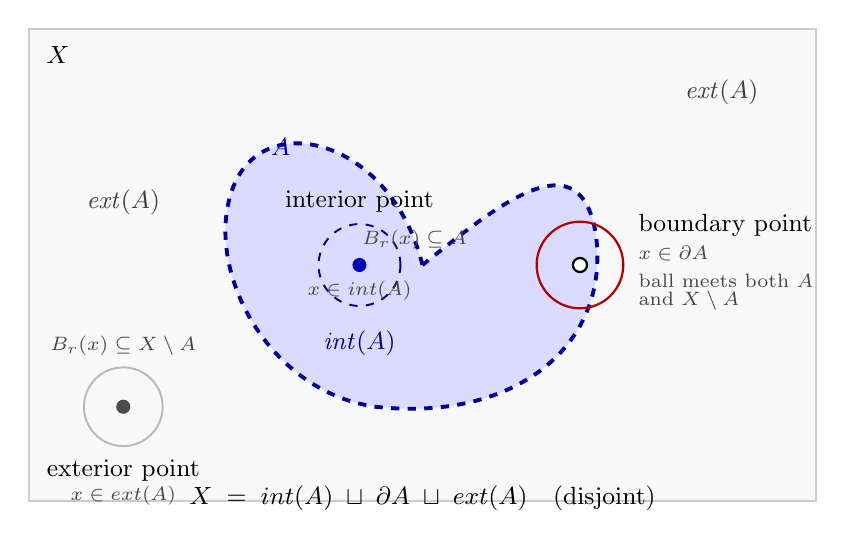
\begin{tikzpicture}[
  dot/.style={circle, fill, inner sep=1.8pt},
  opendot/.style={circle, draw, fill=white, inner sep=1.8pt, line width=0.8pt},
  lbl/.style={font=\small},
  slbl/.style={font=\scriptsize, text=gray!55!black},
  >=stealth
]

% ---- Ambient space X (large rectangle) ----
\fill[gray!5] (-5.0,-3.0) rectangle (5.0,3.0);
\draw[gray!40, line width=0.8pt] (-5.0,-3.0) rectangle (5.0,3.0);
\node[lbl, anchor=north west] at (-4.9, 2.9) {$X$};

% ---- Set A (blob) ----
\fill[blue!14]
  (0, 0)
  .. controls (-0.4, 1.6) and (-2.0, 2.0) .. (-2.4, 1.0)
  .. controls (-2.8, 0.0) and (-2.0,-1.6) .. (-0.6,-1.8)
  .. controls ( 1.2,-2.0) and ( 2.4,-1.0) .. ( 2.2, 0.4)
  .. controls ( 2.0, 1.6) and ( 1.0, 0.8) .. (0, 0)
  -- cycle;

% ---- Boundary (slightly thicker dashed curve) ----
\draw[blue!60!black, line width=1.4pt, dashed]
  (0, 0)
  .. controls (-0.4, 1.6) and (-2.0, 2.0) .. (-2.4, 1.0)
  .. controls (-2.8, 0.0) and (-2.0,-1.6) .. (-0.6,-1.8)
  .. controls ( 1.2,-2.0) and ( 2.4,-1.0) .. ( 2.2, 0.4)
  .. controls ( 2.0, 1.6) and ( 1.0, 0.8) .. (0, 0)
  -- cycle;

% ---- Interior point (well inside A) ----
\coordinate (int) at (-0.8, 0.0);
\node[dot, blue!70!black] at (int) {};
\draw[blue!60!black, dashed, line width=0.7pt] (int) circle (0.52cm);
\node[lbl, anchor=south] at (-0.8, 0.55) {interior point};
\node[slbl, anchor=north] at (-0.8, -0.08) {$x \in \operatorname{int}(A)$};
% small label on ball
\node[slbl] at (-0.8+0.7, 0.32) {$B_r(x) \subseteq A$};

% ---- Boundary point (on the dashed curve) ----
\coordinate (bdy) at (2.0, 0.0);
\node[opendot] at (bdy) {};
\draw[red!70!black, line width=0.8pt] (bdy) circle (0.55cm);
\node[lbl, anchor=west] at (2.62, 0.5) {boundary point};
\node[slbl, anchor=west] at (2.62, 0.15) {$x \in \partial A$};
\node[slbl, anchor=west] at (2.62,-0.2) {ball meets both $A$};
\node[slbl, anchor=west] at (2.62,-0.45) {and $X \setminus A$};

% ---- Exterior point (outside A) ----
\coordinate (ext) at (-3.8, -1.8);
\node[dot, gray!60!black] at (ext) {};
\draw[gray!55, line width=0.7pt] (ext) circle (0.50cm);
\node[lbl, anchor=north] at (-3.8, -2.35) {exterior point};
\node[slbl, anchor=north] at (-3.8, -2.68) {$x \in \operatorname{ext}(A)$};
\node[slbl, anchor=south] at (-3.8, -1.27) {$B_r(x) \subseteq X\setminus A$};

% ---- Region labels ----
\node[lbl, blue!55!black] at (-0.8, -1.0) {\textit{int}$(A)$};
\node[lbl, gray!50!black] at (-3.8, 0.8) {\textit{ext}$(A)$};
\node[lbl, gray!50!black] at (3.8, 2.2) {\textit{ext}$(A)$};
\node[lbl, blue!65!black] at (-1.8, 1.5) {$A$};

% ---- Decomposition formula ----
\node[lbl, anchor=south] at (0, -3.25) {%
  $X \;=\; \operatorname{int}(A) \;\sqcup\; \partial A \;\sqcup\; \operatorname{ext}(A)$%
  \quad (disjoint)};

\end{tikzpicture}
\caption{The interior--boundary--exterior decomposition of a metric space $X$
relative to a set $A$ (shaded blue).
The interior point $x$ has a ball fitting entirely inside $A$.
The boundary point sits on the dashed curve: every ball around it meets both $A$ and $X\setminus A$.
The exterior point has a ball fitting entirely in $X\setminus A$.
Every point of $X$ belongs to exactly one of the three regions.}
\label{fig:ibe-decomposition}
\end{figure}
